%===================================== CHAP 5 =================================

\chapter{Results} \label{results-chapter}

\section{Visualization Tool}

\subsection{Example Networks}

The visualization results were generated using two separate example ANNs. The first network is a simple CNN trained on the MNIST dataset, commonly used as a toy problem. This network is quickly trained from scratch to near to perfect accuracy, which allowed us to show how the visualizations evolve throughout the training progress. The second network is the more advanced VGG16 network. In this case, we used a fully trained model with weights pretrained on ImageNet. Some of the visualizations, for instance the deconvolutional network technique, require a large network with many convolutional layers to demonstrate their full capabilities. Using a fully trained VGG16 model, we could present a second set of visualizations that showcase more complex features, without having to spend a large amount of time training the network. The VGG16 network also allows us to display how the visualizations handle RGB images, compared to the grayscale images of the MNIST dataset. Both networks were implemented following examples provided by Keras, and in the following sections we describe their implementations and training processes in detail.\\

\noindent Note that there are several ways to count the number of layers in a network. Some conventions do not include pooling or flatten layers, or even the input and output layers. To ensure consistency when describing the network architectures, we will define the number of layers as the number of Keras layers, as listed in their documentation, and in the illustrations of the network architectures.

\subsubsection{The MNIST Network}

%870: 'tricycle, trike, velocipede', 0.999541
%972: 'cliff, drop, drop-off', 0.643459
%808: 'sombrero', 0.509112

% something about grayscale images and that the size of input is only 28, 28

The MNIST network is a simple CNN with three convolutional layers including the max pooling layer. The architecture can be seen in \textbf{Fig. \ref{mnist-architecture}}, and was created following an example implementation by Keras. The network consists of 10 layers, where three of these are convolutional layers and two of them fully connected layers, noted as Dense layers in Keras. In addition to an input layer, there are also two dropout layers to prevent overfitting, and a flatten layer to convert the 2D output from the convolutional part to 1D input for the fully connected part. The Keras model is compiled using the Adadelta optimizer and categorical crossentropy loss. \\

\noindent To generate the results, the MNIST network was trained for two epochs with a batch size of 128 and the data shuffled at each epoch. 10 images were extracted from the test data, one for each class (0-9), to be used as visualization images. Then, the training process was repeated using each of the visualization images as input for the visualizations. The visualizations were produced five times during each epoch, in addition to at the very beginning of the training, giving a total of 11 different sets of visualization results for each of the 10 digits. For the deconvolutional network technique, all 32 feature maps of the \texttt{pool} layer were visualized. For deep visualization, all units in \texttt{output} as well as a sample of units from the remaining layers, except the dropout and flatten layers, were included. The deep visualizations were produced with a learning rate of 200 and 50 iterations. The $L_2$ decay, blur interval and blur standard deviation were set to 0.0001, 4 and 1 respectively, matching one of the useful combinations in \textbf{Table \ref{tab:reg_hyperparams}}. The produced visualizations were manually processed, and a representative selection of the resulting visualizations were extracted, presented in section \ref{mnist-vis-results}.

\subsubsection{The VGG16 Network}

The VGG16 network is a significantly deeper CNN consisting of five blocks of 3-4 convolutional layers each, including the max pooling layers, followed by a flatten layer and three fully-connected layers, giving a total of 23 layers. The full architecture can be seen in \textbf{Fig. \ref{vgg-architecture}}. The adopted VGG16 model has weights pretrained on ImageNet and is available through the Keras Applications module. The model was compiled using the RMSprop optimizer and categorical crossentropy loss. \\

As mentioned, the VGG16 network employed was an already fully trained model, thus the results presented using this network only consist of visualizations produced at the very end of the training process. Consequently, there was no training involved in generating the results. For the deconvolutional network technique, the top 20 maximally activated feature maps of \texttt{block5\_pool}, \texttt{block3\_pool} and \texttt{block1\_pool} were visualized using image A. Additionally, the same feature maps of \texttt{block5\_pool} and \texttt{block3\_pool} were visualized using image B and image C. These two images were selected because they are both related to image A in some way. Specifically, image B contains a bicycle similar to the tricycle in image A, and image C contains a woman similar to the girl in image A. For deep visualization, 20 classes were selected in \texttt{output}, as well as a sample of units from \texttt{fc1}, \texttt{fc2} and each of the pooling layers. The deep visualizations were produced with a learning rate of 2500 and 500 iterations. The $L_2$ decay, blur interval and blur standard deviation were set to 0.0001, 4 and 1 respectively, matching one of the useful combinations in \textbf{Table \ref{tab:reg_hyperparams}}. The produced visualizations were manually processed, and a representative selection of the resulting visualizations were extracted, presented in section \ref{vgg-vis-results}.

\begin{figure}
    \begin{minipage}{0.5\textwidth}
        \centering
            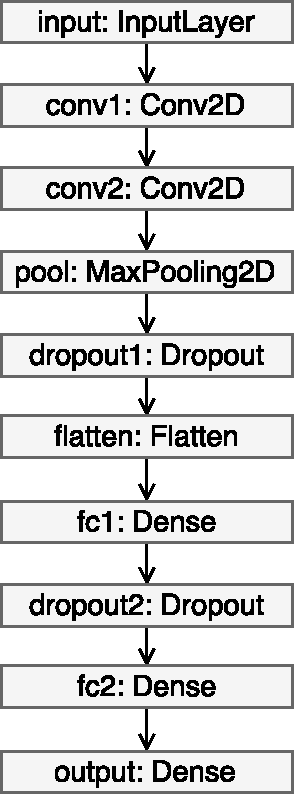
\includegraphics[width=0.6\textwidth]{fig/mnist_keras.pdf}
            \caption{Architecture of the MNIST network}
            \label{mnist-architecture}
    \end{minipage}
    \begin{minipage}{0.4\textwidth}
        \centering
            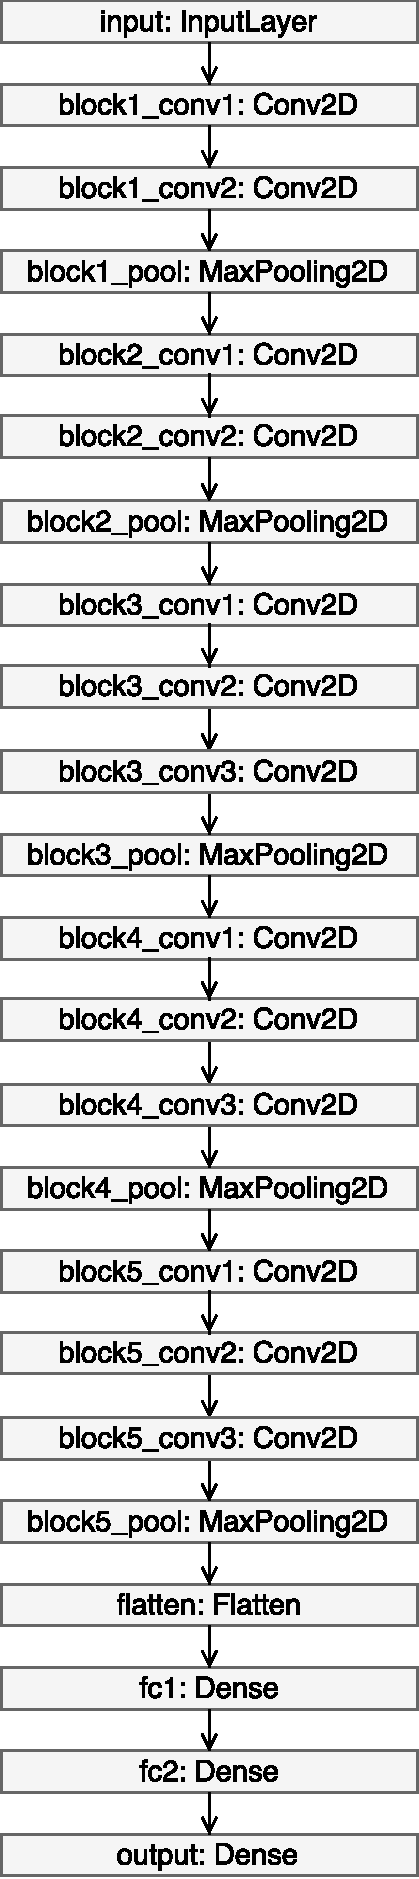
\includegraphics[width=0.7\textwidth]{fig/vgg_keras.pdf}
            \caption{Architecture of the VGG network}
            \label{vgg-architecture}
    \end{minipage}
\end{figure}

\subsection{MNIST Visualization Results} \label{mnist-vis-results}

\subsubsection{Training Progress}

\subsubsection{Layer Activations}

\begin{figure}
\begin{center}
\begin{tabular}{c}
\begingroup
\captionsetup[subfigure]{width=1in}
\subfloat[Input layer]{\makebox[1in][c]{
\includegraphics[width = 0.4in]{fig/results/input_mnist/test0.png}}}\endgroup \\
\subfloat[Convolution layer 1]{\frame{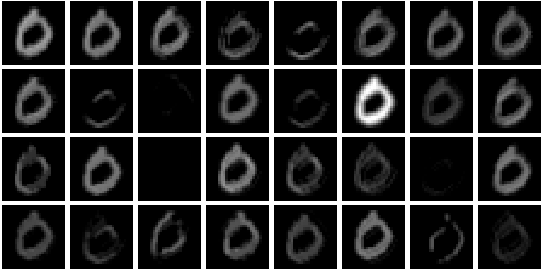
\includegraphics[width=0.6\textwidth]{fig/results/layeract_mnist/all_layers/layer_act_mnist_0_10_conv2d_1.png}}} \\
\subfloat[Convolution layer 2]{\frame{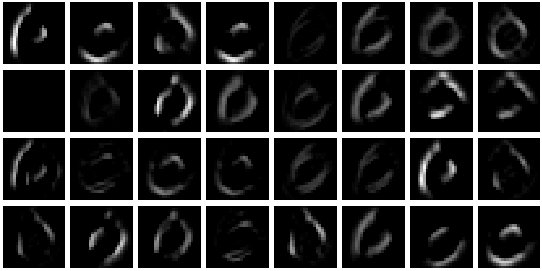
\includegraphics[width=0.6\textwidth]{fig/results/layeract_mnist/all_layers/layer_act_mnist_0_10_conv2d_2.png}}} \\
\subfloat[Max pooling layer]{\frame{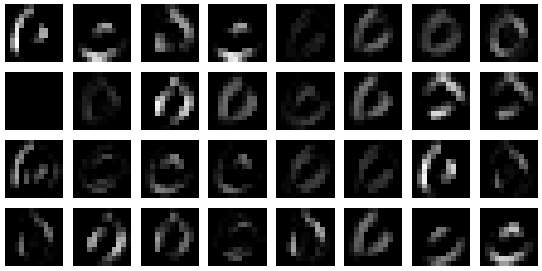
\includegraphics[width=0.5\textwidth]{fig/results/layeract_mnist/all_layers/layer_act_mnist_0_10_max_pooling2d_1.png}}} \\
\subfloat[Fully connected layer 1]{\frame{
\includegraphics[width=\textwidth]{fig/results/layeract_mnist/all_layers/layer_act_mnist_0_10_dense_1.png}}} \\
\subfloat[Fully connected layer 2]{\frame{
\includegraphics[width=\textwidth]{fig/results/layeract_mnist/all_layers/layer_act_mnist_0_10_dense_2.png}}} \\
\subfloat[Fully connected layer 3 (output layer)]{\frame{
\includegraphics[width=0.3\textwidth]{fig/results/layeract_mnist/all_layers/layer_act_mnist_0_10_dense_3.png}}} \\
\end{tabular}
\caption[Layer activations for all MNIST layers]{Layer activations for all layers of the MNIST network, excluding flatten and dropout layers, for input 0.}
\end{center}
\end{figure}

\begin{figure}
\begin{center}
\begin{tabular}{c}
\begingroup
\captionsetup[subfigure]{width=1in}
\subfloat[0]{\frame{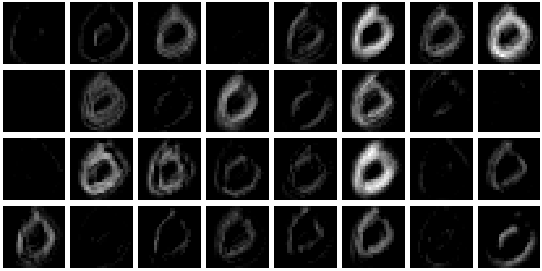
\includegraphics[width=0.6\textwidth]{fig/results/layeract_mnist/layer_act_mnist_0_0_conv2d_2.png}}} \\
\subfloat[5]{\frame{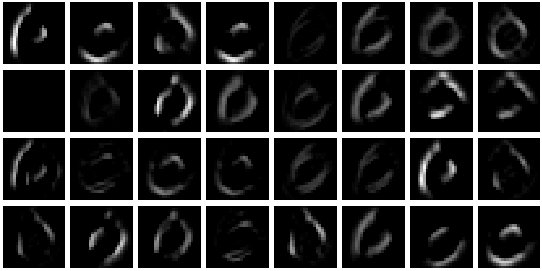
\includegraphics[width=0.6\textwidth]{fig/results/layeract_mnist/all_layers/layer_act_mnist_0_10_conv2d_2.png}}} \\
\end{tabular}
\caption[Layer activations for all MNIST layers]{Layer activations for all layers of the MNIST network, excluding flatten and dropout layers, for input 0.}
\end{center}
\end{figure}

\subsubsection{Saliency Maps}

\begin{figure}
\begin{center}
\begin{tabular}{ccccccc}
\textbf{Input} & \textbf{0} & \textbf{2} & \textbf{4} & \textbf{6} & \textbf{8} & \textbf{10} \\
\subfloat{
\includegraphics[width = 0.5in]{fig/results/input_mnist/test0.png}} &
\subfloat{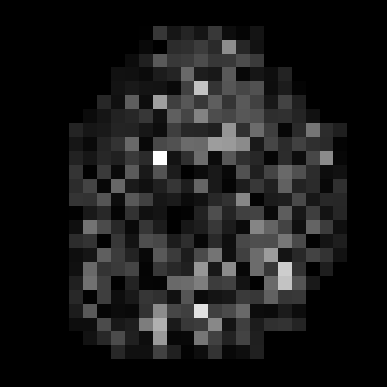
\includegraphics[width = 0.5in]{fig/results/saliency_mnist/saliency_mnist_0_0.png}} &
\subfloat{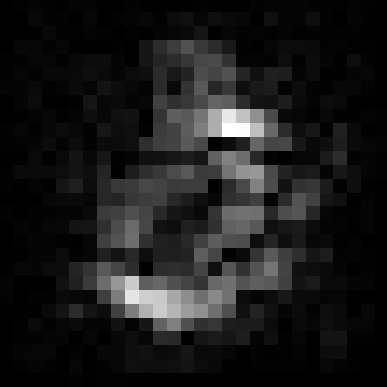
\includegraphics[width = 0.5in]{fig/results/saliency_mnist/saliency_mnist_0_2.png}} &
\subfloat{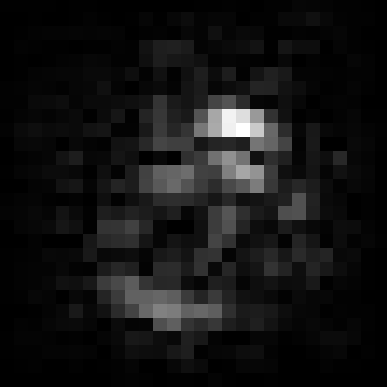
\includegraphics[width = 0.5in]{fig/results/saliency_mnist/saliency_mnist_0_4.png}} &
\subfloat{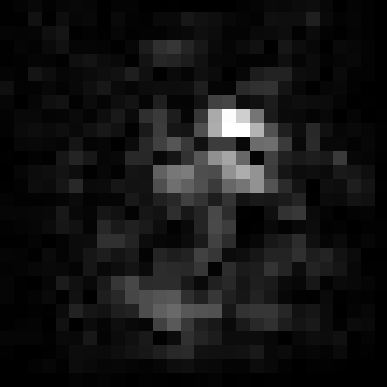
\includegraphics[width = 0.5in]{fig/results/saliency_mnist/saliency_mnist_0_6.png}} &
\subfloat{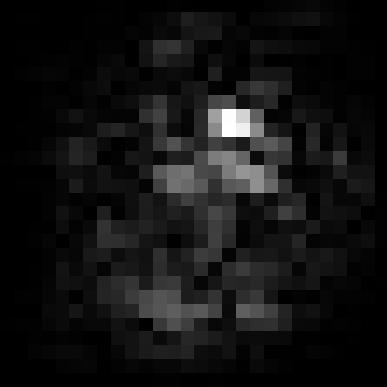
\includegraphics[width = 0.5in]{fig/results/saliency_mnist/saliency_mnist_0_8.png}} &
\subfloat{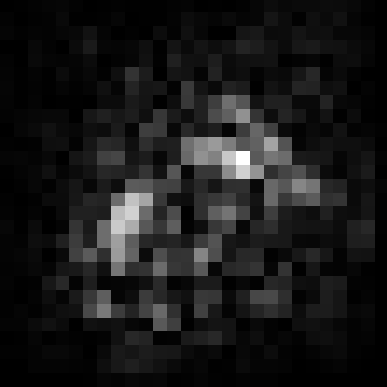
\includegraphics[width = 0.5in]{fig/results/saliency_mnist/saliency_mnist_0_10.png}} \\
\subfloat{
\includegraphics[width = 0.5in]{fig/results/input_mnist/test1.png}} & 
\subfloat{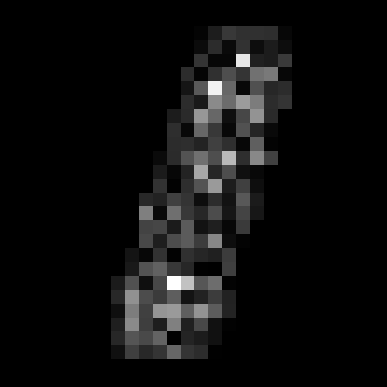
\includegraphics[width = 0.5in]{fig/results/saliency_mnist/saliency_mnist_1_0.png}} &
\subfloat{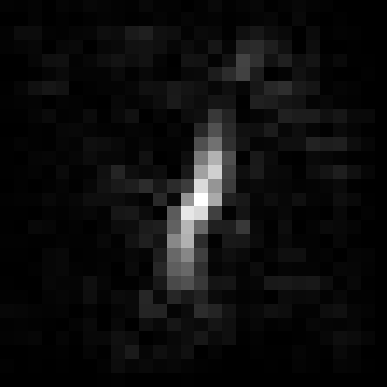
\includegraphics[width = 0.5in]{fig/results/saliency_mnist/saliency_mnist_1_2.png}} &
\subfloat{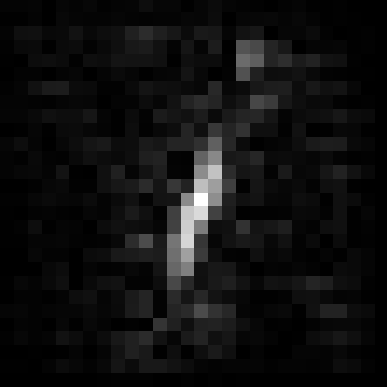
\includegraphics[width = 0.5in]{fig/results/saliency_mnist/saliency_mnist_1_4.png}} &
\subfloat{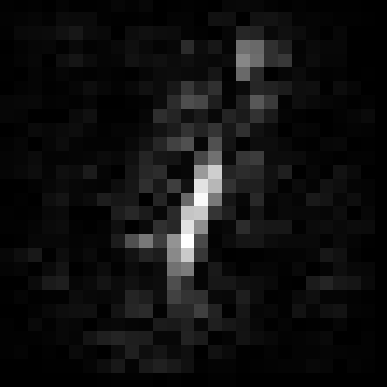
\includegraphics[width = 0.5in]{fig/results/saliency_mnist/saliency_mnist_1_6.png}} &
\subfloat{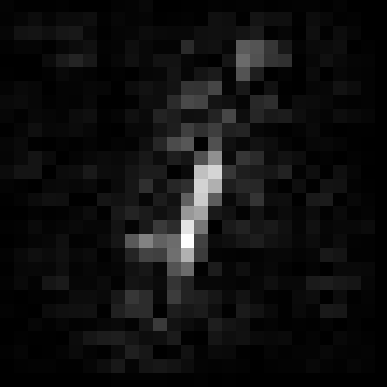
\includegraphics[width = 0.5in]{fig/results/saliency_mnist/saliency_mnist_1_8.png}} &
\subfloat{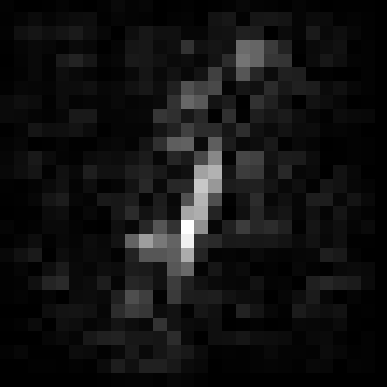
\includegraphics[width = 0.5in]{fig/results/saliency_mnist/saliency_mnist_1_10.png}} \\
\subfloat{
\includegraphics[width = 0.5in]{fig/results/input_mnist/test2.png}} &
\subfloat{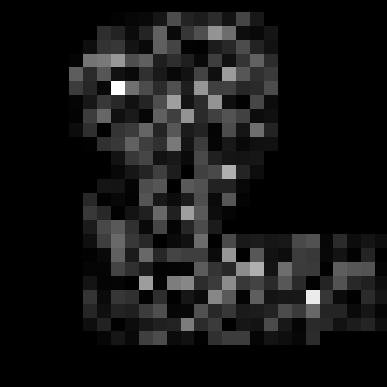
\includegraphics[width = 0.5in]{fig/results/saliency_mnist/saliency_mnist_2_0.png}} &
\subfloat{
\includegraphics[width = 0.5in]{fig/results/saliency_mnist/saliency_mnist_2_2.png}} &
\subfloat{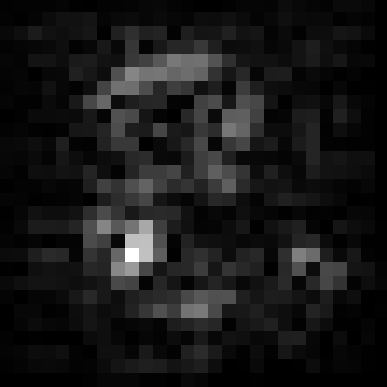
\includegraphics[width = 0.5in]{fig/results/saliency_mnist/saliency_mnist_2_4.png}} &
\subfloat{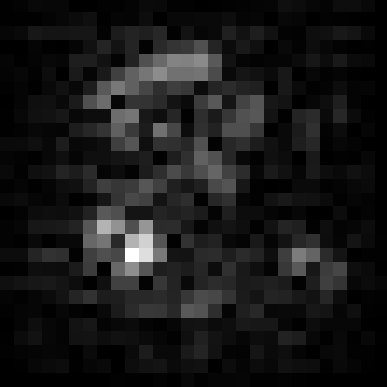
\includegraphics[width = 0.5in]{fig/results/saliency_mnist/saliency_mnist_2_6.png}} &
\subfloat{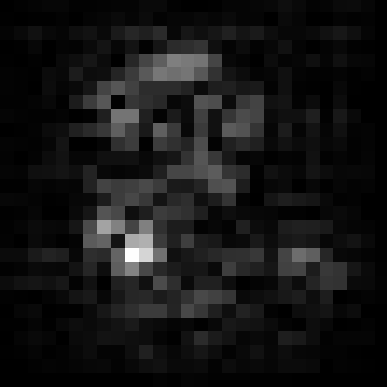
\includegraphics[width = 0.5in]{fig/results/saliency_mnist/saliency_mnist_2_8.png}} &
\subfloat{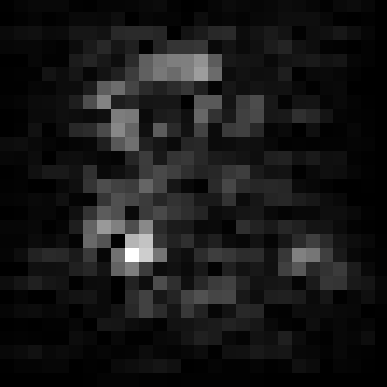
\includegraphics[width = 0.5in]{fig/results/saliency_mnist/saliency_mnist_2_10.png}} \\   
\subfloat{
\includegraphics[width = 0.5in]{fig/results/input_mnist/test3.png}} &
\subfloat{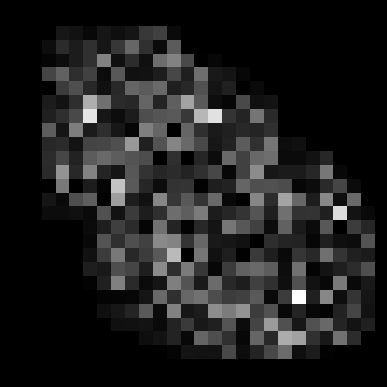
\includegraphics[width = 0.5in]{fig/results/saliency_mnist/saliency_mnist_3_0.png}} &
\subfloat{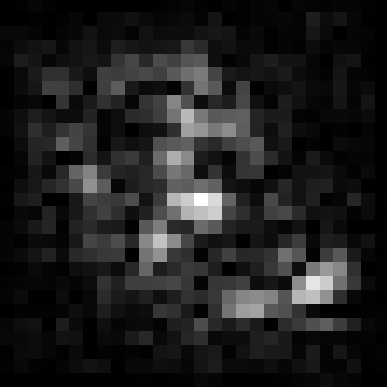
\includegraphics[width = 0.5in]{fig/results/saliency_mnist/saliency_mnist_3_2.png}} &
\subfloat{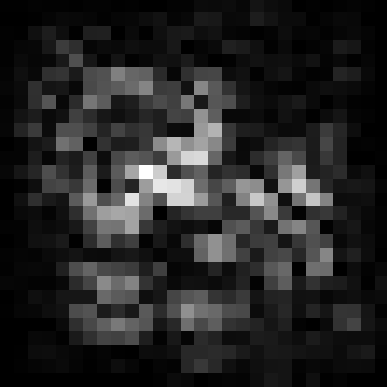
\includegraphics[width = 0.5in]{fig/results/saliency_mnist/saliency_mnist_3_4.png}} &
\subfloat{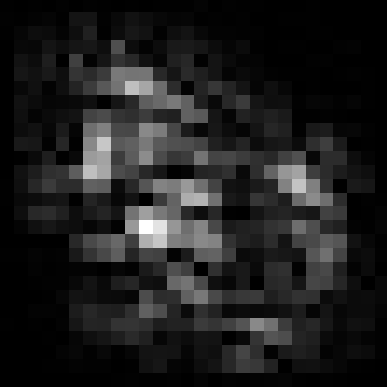
\includegraphics[width = 0.5in]{fig/results/saliency_mnist/saliency_mnist_3_6.png}} &
\subfloat{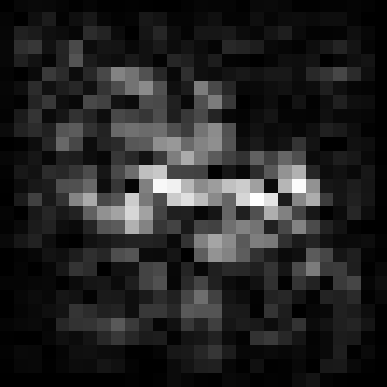
\includegraphics[width = 0.5in]{fig/results/saliency_mnist/saliency_mnist_3_8.png}} &
\subfloat{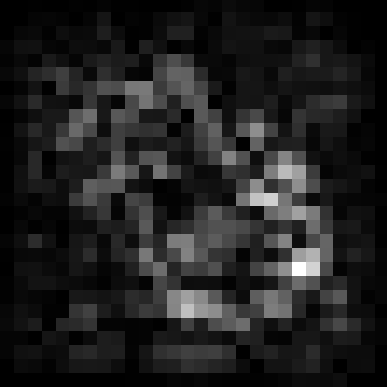
\includegraphics[width = 0.5in]{fig/results/saliency_mnist/saliency_mnist_3_10.png}} \\
\subfloat{
\includegraphics[width = 0.5in]{fig/results/input_mnist/test4.png}} &
\subfloat{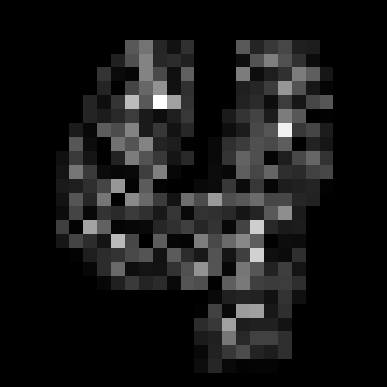
\includegraphics[width = 0.5in]{fig/results/saliency_mnist/saliency_mnist_4_0.png}} &
\subfloat{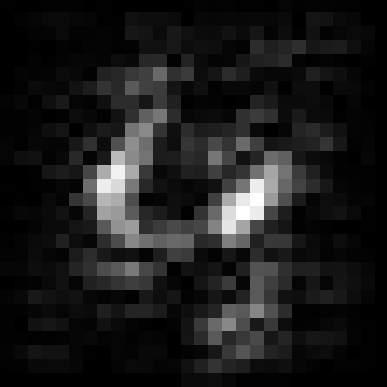
\includegraphics[width = 0.5in]{fig/results/saliency_mnist/saliency_mnist_4_2.png}} &
\subfloat{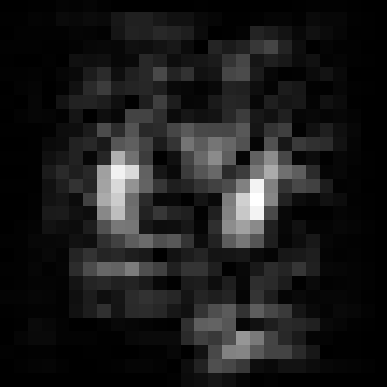
\includegraphics[width = 0.5in]{fig/results/saliency_mnist/saliency_mnist_4_4.png}} &
\subfloat{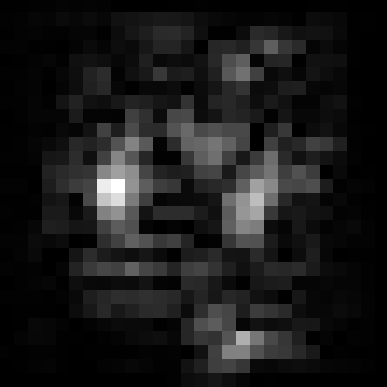
\includegraphics[width = 0.5in]{fig/results/saliency_mnist/saliency_mnist_4_6.png}} &
\subfloat{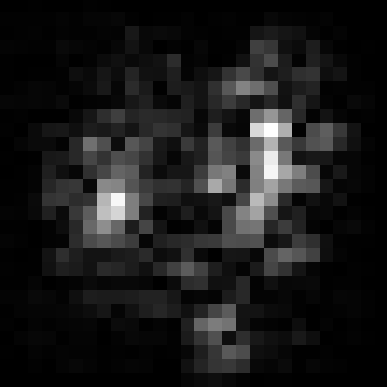
\includegraphics[width = 0.5in]{fig/results/saliency_mnist/saliency_mnist_4_8.png}} &
\subfloat{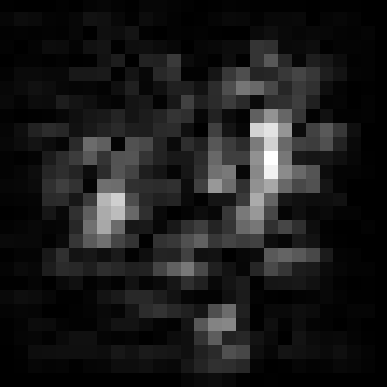
\includegraphics[width = 0.5in]{fig/results/saliency_mnist/saliency_mnist_4_10.png}} \\
\subfloat{
\includegraphics[width = 0.5in]{fig/results/input_mnist/test5.png}} &
\subfloat{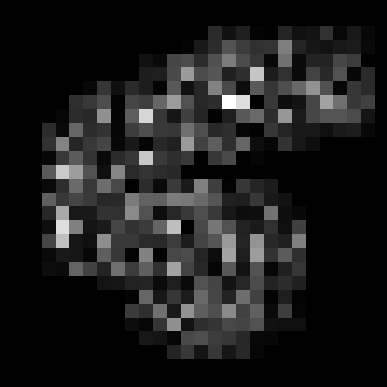
\includegraphics[width = 0.5in]{fig/results/saliency_mnist/saliency_mnist_5_0.png}} &
\subfloat{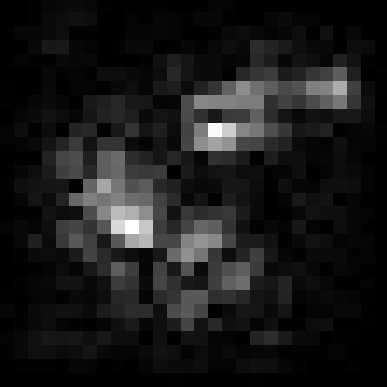
\includegraphics[width = 0.5in]{fig/results/saliency_mnist/saliency_mnist_5_2.png}} &
\subfloat{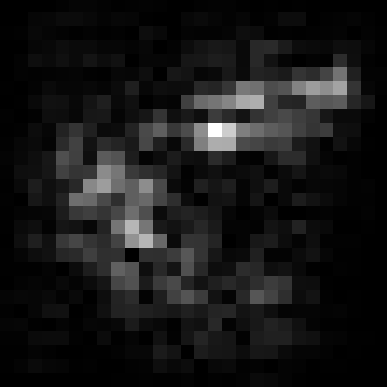
\includegraphics[width = 0.5in]{fig/results/saliency_mnist/saliency_mnist_5_4.png}} &
\subfloat{\includegraphics[width = 0.5in]{fig/results/saliency_mnist/saliency_mnist_5_6.png}} &
\subfloat{\includegraphics[width = 0.5in]{fig/results/saliency_mnist/saliency_mnist_5_8.png}} &
\subfloat{\includegraphics[width = 0.5in]{fig/results/saliency_mnist/saliency_mnist_5_10.png}} \\
\subfloat{\includegraphics[width = 0.5in]{fig/results/input_mnist/test6.png}} &
\subfloat{\includegraphics[width = 0.5in]{fig/results/saliency_mnist/saliency_mnist_6_0.png}} &
\subfloat{\includegraphics[width = 0.5in]{fig/results/saliency_mnist/saliency_mnist_6_2.png}} &
\subfloat{\includegraphics[width = 0.5in]{fig/results/saliency_mnist/saliency_mnist_6_4.png}} &
\subfloat{\includegraphics[width = 0.5in]{fig/results/saliency_mnist/saliency_mnist_6_6.png}} &
\subfloat{\includegraphics[width = 0.5in]{fig/results/saliency_mnist/saliency_mnist_6_8.png}} &
\subfloat{\includegraphics[width = 0.5in]{fig/results/saliency_mnist/saliency_mnist_6_10.png}} \\
\subfloat{\includegraphics[width = 0.5in]{fig/results/input_mnist/test7.png}} &
\subfloat{\includegraphics[width = 0.5in]{fig/results/saliency_mnist/saliency_mnist_7_0.png}} &
\subfloat{\includegraphics[width = 0.5in]{fig/results/saliency_mnist/saliency_mnist_7_2.png}} &
\subfloat{\includegraphics[width = 0.5in]{fig/results/saliency_mnist/saliency_mnist_7_4.png}} &
\subfloat{\includegraphics[width = 0.5in]{fig/results/saliency_mnist/saliency_mnist_7_6.png}} &
\subfloat{\includegraphics[width = 0.5in]{fig/results/saliency_mnist/saliency_mnist_7_8.png}} &
\subfloat{\includegraphics[width = 0.5in]{fig/results/saliency_mnist/saliency_mnist_7_10.png}} \\
\subfloat{\includegraphics[width = 0.5in]{fig/results/input_mnist/test8.png}} &
\subfloat{\includegraphics[width = 0.5in]{fig/results/saliency_mnist/saliency_mnist_8_0.png}} &
\subfloat{\includegraphics[width = 0.5in]{fig/results/saliency_mnist/saliency_mnist_8_2.png}} &
\subfloat{\includegraphics[width = 0.5in]{fig/results/saliency_mnist/saliency_mnist_8_4.png}} &
\subfloat{\includegraphics[width = 0.5in]{fig/results/saliency_mnist/saliency_mnist_8_6.png}} &
\subfloat{\includegraphics[width = 0.5in]{fig/results/saliency_mnist/saliency_mnist_8_8.png}} &
\subfloat{\includegraphics[width = 0.5in]{fig/results/saliency_mnist/saliency_mnist_8_10.png}} \\
\subfloat{\includegraphics[width = 0.5in]{fig/results/input_mnist/test9.png}} &
\subfloat{\includegraphics[width = 0.5in]{fig/results/saliency_mnist/saliency_mnist_9_0.png}} &
\subfloat{\includegraphics[width = 0.5in]{fig/results/saliency_mnist/saliency_mnist_9_2.png}} &
\subfloat{\includegraphics[width = 0.5in]{fig/results/saliency_mnist/saliency_mnist_9_4.png}} &
\subfloat{\includegraphics[width = 0.5in]{fig/results/saliency_mnist/saliency_mnist_9_6.png}} &
\subfloat{\includegraphics[width = 0.5in]{fig/results/saliency_mnist/saliency_mnist_9_8.png}} &
\subfloat{\includegraphics[width = 0.5in]{fig/results/saliency_mnist/saliency_mnist_9_10.png}}
\end{tabular}
\caption[Saliency maps for MNIST network]{Saliency maps for the MNIST network with input 0-9. Input image is shown in the first column, the rest are samples taken over a period of two epochs. Stage 0 is produced before training has started.}
\end{center}
\end{figure}

\subsubsection{Deconvolutional Network}

\subsubsection{Deep Visualization}

\begin{figure}
\begin{center}
\begin{tabular}{cccccc}
\textbf{Example} & \textbf{1} & \textbf{5} & \textbf{10 v.1} & \textbf{10 v.2} & \textbf{10 v.3}\\
\subfloat{\includegraphics[width = 0.5in]{fig/results/input_mnist/test0.png}} &
\subfloat{\includegraphics[width = 0.5in]{fig/results/deepvis_mnist/deepvis_mnist_0_1_dense_3_0.png}} &
\subfloat{\includegraphics[width = 0.5in]{fig/results/deepvis_mnist/deepvis_mnist_0_5_dense_3_0.png}} & \subfloat{\includegraphics[width = 0.5in]{fig/results/deepvis_mnist/deepvis_mnist_0_10_dense_3_0.png}} &
\subfloat{\includegraphics[width = 0.5in]{fig/results/deepvis_mnist/other_numbers/deepvis_mnist_1_10_dense_3_0.png}} &
\subfloat{\includegraphics[width = 0.5in]{fig/results/deepvis_mnist/other_numbers/deepvis_mnist_2_10_dense_3_0.png}} \\
\subfloat{\includegraphics[width = 0.5in]{fig/results/input_mnist/test1.png}} &
\subfloat{\includegraphics[width = 0.5in]{fig/results/deepvis_mnist/deepvis_mnist_0_1_dense_3_1.png}} &
\subfloat{\includegraphics[width = 0.5in]{fig/results/deepvis_mnist/deepvis_mnist_0_5_dense_3_1.png}} & \subfloat{\includegraphics[width = 0.5in]{fig/results/deepvis_mnist/deepvis_mnist_0_10_dense_3_1.png}} &
\subfloat{\includegraphics[width = 0.5in]{fig/results/deepvis_mnist/other_numbers/deepvis_mnist_1_10_dense_3_1.png}} &
\subfloat{\includegraphics[width = 0.5in]{fig/results/deepvis_mnist/other_numbers/deepvis_mnist_2_10_dense_3_1.png}} \\
\subfloat{\includegraphics[width = 0.5in]{fig/results/input_mnist/test2.png}} &
\subfloat{\includegraphics[width = 0.5in]{fig/results/deepvis_mnist/deepvis_mnist_0_1_dense_3_2.png}} &
\subfloat{\includegraphics[width = 0.5in]{fig/results/deepvis_mnist/deepvis_mnist_0_5_dense_3_2.png}} & \subfloat{\includegraphics[width = 0.5in]{fig/results/deepvis_mnist/deepvis_mnist_0_10_dense_3_2.png}} &
\subfloat{\includegraphics[width = 0.5in]{fig/results/deepvis_mnist/other_numbers/deepvis_mnist_1_10_dense_3_2.png}} &
\subfloat{\includegraphics[width = 0.5in]{fig/results/deepvis_mnist/other_numbers/deepvis_mnist_2_10_dense_3_2.png}} \\
\subfloat{\includegraphics[width = 0.5in]{fig/results/input_mnist/test3.png}} &
\subfloat{\includegraphics[width = 0.5in]{fig/results/deepvis_mnist/deepvis_mnist_0_1_dense_3_3.png}} &
\subfloat{\includegraphics[width = 0.5in]{fig/results/deepvis_mnist/deepvis_mnist_0_5_dense_3_3.png}} & \subfloat{\includegraphics[width = 0.5in]{fig/results/deepvis_mnist/deepvis_mnist_0_10_dense_3_3.png}} &
\subfloat{\includegraphics[width = 0.5in]{fig/results/deepvis_mnist/other_numbers/deepvis_mnist_1_10_dense_3_3.png}} &
\subfloat{\includegraphics[width = 0.5in]{fig/results/deepvis_mnist/other_numbers/deepvis_mnist_2_10_dense_3_3.png}} \\
\subfloat{\includegraphics[width = 0.5in]{fig/results/input_mnist/test4.png}} &
\subfloat{\includegraphics[width = 0.5in]{fig/results/deepvis_mnist/deepvis_mnist_0_1_dense_3_4.png}} &
\subfloat{\includegraphics[width = 0.5in]{fig/results/deepvis_mnist/deepvis_mnist_0_5_dense_3_4.png}} & \subfloat{\includegraphics[width = 0.5in]{fig/results/deepvis_mnist/deepvis_mnist_0_10_dense_3_4.png}} &
\subfloat{\includegraphics[width = 0.5in]{fig/results/deepvis_mnist/other_numbers/deepvis_mnist_1_10_dense_3_4.png}} &
\subfloat{\includegraphics[width = 0.5in]{fig/results/deepvis_mnist/other_numbers/deepvis_mnist_2_10_dense_3_4.png}} \\
\subfloat{\includegraphics[width = 0.5in]{fig/results/input_mnist/test5.png}} &
\subfloat{\includegraphics[width = 0.5in]{fig/results/deepvis_mnist/deepvis_mnist_0_1_dense_3_5.png}} &
\subfloat{\includegraphics[width = 0.5in]{fig/results/deepvis_mnist/deepvis_mnist_0_5_dense_3_5.png}} & \subfloat{\includegraphics[width = 0.5in]{fig/results/deepvis_mnist/deepvis_mnist_0_10_dense_3_5.png}} &
\subfloat{\includegraphics[width = 0.5in]{fig/results/deepvis_mnist/other_numbers/deepvis_mnist_1_10_dense_3_5.png}} &
\subfloat{\includegraphics[width = 0.5in]{fig/results/deepvis_mnist/other_numbers/deepvis_mnist_2_10_dense_3_5.png}} \\
\subfloat{\includegraphics[width = 0.5in]{fig/results/input_mnist/test6.png}} &
\subfloat{\includegraphics[width = 0.5in]{fig/results/deepvis_mnist/deepvis_mnist_0_1_dense_3_6.png}} &
\subfloat{\includegraphics[width = 0.5in]{fig/results/deepvis_mnist/deepvis_mnist_0_5_dense_3_6.png}} & \subfloat{\includegraphics[width = 0.5in]{fig/results/deepvis_mnist/deepvis_mnist_0_10_dense_3_6.png}} &
\subfloat{\includegraphics[width = 0.5in]{fig/results/deepvis_mnist/other_numbers/deepvis_mnist_1_10_dense_3_6.png}} &
\subfloat{\includegraphics[width = 0.5in]{fig/results/deepvis_mnist/other_numbers/deepvis_mnist_2_10_dense_3_6.png}} \\
\subfloat{\includegraphics[width = 0.5in]{fig/results/input_mnist/test7.png}} &
\subfloat{\includegraphics[width = 0.5in]{fig/results/deepvis_mnist/deepvis_mnist_0_1_dense_3_7.png}} &
\subfloat{\includegraphics[width = 0.5in]{fig/results/deepvis_mnist/deepvis_mnist_0_5_dense_3_7.png}} & \subfloat{\includegraphics[width = 0.5in]{fig/results/deepvis_mnist/deepvis_mnist_0_10_dense_3_7.png}} &
\subfloat{\includegraphics[width = 0.5in]{fig/results/deepvis_mnist/other_numbers/deepvis_mnist_1_10_dense_3_7.png}} &
\subfloat{\includegraphics[width = 0.5in]{fig/results/deepvis_mnist/other_numbers/deepvis_mnist_2_10_dense_3_7.png}} \\
\subfloat{\includegraphics[width = 0.5in]{fig/results/input_mnist/test8.png}} &
\subfloat{\includegraphics[width = 0.5in]{fig/results/deepvis_mnist/deepvis_mnist_0_1_dense_3_8.png}} &
\subfloat{\includegraphics[width = 0.5in]{fig/results/deepvis_mnist/deepvis_mnist_0_5_dense_3_8.png}} & \subfloat{\includegraphics[width = 0.5in]{fig/results/deepvis_mnist/deepvis_mnist_0_10_dense_3_8.png}} &
\subfloat{\includegraphics[width = 0.5in]{fig/results/deepvis_mnist/other_numbers/deepvis_mnist_1_10_dense_3_8.png}} &
\subfloat{\includegraphics[width = 0.5in]{fig/results/deepvis_mnist/other_numbers/deepvis_mnist_2_10_dense_3_8.png}} \\
\subfloat{\includegraphics[width = 0.5in]{fig/results/input_mnist/test9.png}} &
\subfloat{\includegraphics[width = 0.5in]{fig/results/deepvis_mnist/deepvis_mnist_0_1_dense_3_9.png}} &
\subfloat{\includegraphics[width = 0.5in]{fig/results/deepvis_mnist/deepvis_mnist_0_5_dense_3_9.png}} & \subfloat{\includegraphics[width = 0.5in]{fig/results/deepvis_mnist/deepvis_mnist_0_10_dense_3_9.png}} &
\subfloat{\includegraphics[width = 0.5in]{fig/results/deepvis_mnist/other_numbers/deepvis_mnist_1_10_dense_3_9.png}} &
\subfloat{\includegraphics[width = 0.5in]{fig/results/deepvis_mnist/other_numbers/deepvis_mnist_2_10_dense_3_9.png}} \\
\end{tabular}
\caption[Deep visualization of output layer of MNIST network]{Deep visualization of the output layer for all classes. An example image from each class is shown in the first column. Column 2-4 shows samples taken over a period of two epochs. The last three columns show the variations of using the deep visualization technique.}
\end{center}
\end{figure}

\begin{figure}
\begin{center}
\begin{tabular}{ccccc}
\subfloat[Unit 0]{\includegraphics[width = 0.5in]{fig/results/deepvis_mnist/other_dense/deepvis_mnist_0_10_dense_2_0}} & 
\subfloat[Unit 24]{\includegraphics[width = 0.5in]{fig/results/deepvis_mnist/other_dense/deepvis_mnist_0_10_dense_2_8}} &
\subfloat[Unit 8]{\includegraphics[width = 0.5in]{fig/results/deepvis_mnist/other_dense/deepvis_mnist_0_10_dense_2_24}} & 
\subfloat[Unit 40]{\includegraphics[width = 0.5in]{fig/results/deepvis_mnist/other_dense/deepvis_mnist_0_10_dense_2_40}} & 
\subfloat[Unit 56]{\includegraphics[width = 0.5in]{fig/results/deepvis_mnist/other_dense/deepvis_mnist_0_10_dense_2_56}} \\
\end{tabular}
\caption[Deepvis dense 2]{Deep visualization of some of the units in the second fully connected layer, i.e. the layer before the output layer.}
\end{center}
\end{figure}

\begin{figure}
\begin{center}
\begin{tabular}{ccc}
\subfloat[Unit 0]{\includegraphics[width = 0.5in]{fig/results/deepvis_mnist/other_dense/deepvis_mnist_0_10_dense_1_0}} & 
\subfloat[Unit 32]{\includegraphics[width = 0.5in]{fig/results/deepvis_mnist/other_dense/deepvis_mnist_0_10_dense_1_32}} &
\subfloat[Unit 96]{\includegraphics[width = 0.5in]{fig/results/deepvis_mnist/other_dense/deepvis_mnist_0_10_dense_1_96}} \\ 
\end{tabular}
\caption[Deepvis dense 1]{Deep visualization of some of the units in the first fully connected layer.}
\end{center}
\end{figure}

\subsection{VGG16 Visualization Results} \label{vgg-vis-results}

\subsubsection{Training Progress}

\subsubsection{Layer Activations}

\subsubsection{Saliency Maps}

\subsubsection{Deconvolutional Network}

\begin{figure}
\begin{center}

\subfloat[Input image]{\includegraphics[width = 1.5in]{fig/results/input_vgg/girlonbike_resized.JPEG}\label{input-img1}}

\begin{tabular}{ccc}
\subfloat[Feature map 108]{\includegraphics[width = 1.5in]{fig/results/deconv_vgg/block5/deconvolution_keras_deconv_0_block5_pool_108.png}} & 
\subfloat[Feature map 348]{\includegraphics[width = 1.5in]{fig/results/deconv_vgg/block5/deconvolution_keras_deconv_0_block5_pool_348.png}} &
\subfloat[Feature map 380]{\includegraphics[width = 1.5in]{fig/results/deconv_vgg/block5/deconvolution_keras_deconv_0_block5_pool_380.png}} \\
\subfloat[Feature map 422]{\includegraphics[width = 1.5in]{fig/results/deconv_vgg/block5/deconvolution_keras_deconv_0_block5_pool_422.png}} &
\subfloat[Feature map 450]{\includegraphics[width = 1.5in]{fig/results/deconv_vgg/block5/deconvolution_keras_deconv_0_block5_pool_450.png}} &
\subfloat[Feature map 459]{\includegraphics[width = 1.5in]{fig/results/deconv_vgg/block5/deconvolution_keras_deconv_0_block5_pool_459.png}} \\
\end{tabular}
\caption[Deconv. block 5]{Visualizations using a deconvolutional network on feature maps in the max pooling layer of block 5. Input image seen in \textbf{a}. A selection of feature maps from the top 20 maximally activated feature maps seen in \textbf{b}-\textbf{g}.}
\end{center}
\end{figure}

\begin{figure}
\begin{center}
\begin{tabular}{ccc}
\subfloat[Input image]{\includegraphics[width = 1.5in]{fig/results/input_vgg/biking_resized.JPEG}\label{input-img2}} &
\subfloat[Feature map 348]{\includegraphics[width = 1.5in]{fig/results/deconv_vgg/other_block5/deconvolution_keras_deconv_0_block5_pool_348.png}} &
\subfloat[Feature map 348 of \textbf{Fig. \ref{input-img1}}]{\includegraphics[width = 1.5in]{fig/results/deconv_vgg/block5/deconvolution_keras_deconv_0_block5_pool_348.png}} \\
\subfloat[Input image]{\includegraphics[width = 1.5in]{fig/results/input_vgg/girl_resized.JPEG}} &
\subfloat[Feature map 380]{\includegraphics[width = 1.5in]{fig/results/deconv_vgg/other_block5/deconvolution_keras_deconv2_0_block5_pool_380.png}} &
\subfloat[Feature map 380 of \textbf{Fig. \ref{input-img1}}]{\includegraphics[width = 1.5in]{fig/results/deconv_vgg/block5/deconvolution_keras_deconv_0_block5_pool_380.png}} \\
\end{tabular}
\caption[Comparison of deconv. block 5]{Comparison of visualizations using a deconvolutional network for specific feature maps in the max pooling layer of block 5. Input images seen in \textbf{a} and \textbf{d}. Visualizations of their feature maps in \textbf{b} and \textbf{c}, with the corresponding feature map visualizations for \textbf{Fig. \ref{input-img1}} in \textbf{c} and \textbf{f}.}
\end{center}
\end{figure}

\begin{figure}
\begin{center}
\begin{tabular}{cccc}
\textbf{Input image} & \textbf{Feature map 25} & \textbf{Feature map 26} & \textbf{Feature map 171} \\
\subfloat{\includegraphics[width = 1.0in]{fig/results/input_vgg/girlonbike_resized.JPEG}} &
\subfloat{\includegraphics[width = 1.0in]{fig/results/deconv_vgg/block3/deconvolution_keras_deconv_block3_0_block3_pool_25.png}} &
\subfloat{\includegraphics[width = 1.0in]{fig/results/deconv_vgg/block3/deconvolution_keras_deconv_block3_0_block3_pool_26.png}} &
\subfloat{\includegraphics[width = 1.0in]{fig/results/deconv_vgg/block3/deconvolution_keras_deconv_block3_0_block3_pool_171.png}} \\
\subfloat{\includegraphics[width = 1.0in]{fig/results/input_vgg/biking_resized.JPEG}} &
\subfloat{\includegraphics[width = 1.0in]{fig/results/deconv_vgg/block3/deconvolution_keras_deconv_block3_specific_0_block3_pool_25.png}} &
\subfloat{\includegraphics[width = 1.0in]{fig/results/deconv_vgg/block3/deconvolution_keras_deconv_block3_specific_0_block3_pool_26.png}} &
\subfloat{\includegraphics[width = 1.0in]{fig/results/deconv_vgg/block3/deconvolution_keras_deconv_block3_specific_0_block3_pool_171.png}} \\
\end{tabular}
\caption[Comparision of deconv. block 3]{Comparison of visualizations using a deconvolutional network for feature maps in the max pooling layer of block 3. Input images seen in the first column. Visualization of their corresponding feature maps in columns 2-4. Feature maps on the top row are selected from the top 20 maximally activated feature maps.}
\end{center}
\end{figure}

\begin{figure}
\begin{center}
\begin{tabular}{cccccccccc}
\subfloat[0]{\frame{\includegraphics[width = 0.3in]{fig/results/deconv_vgg/block1/deconvolution_keras_deconv_block1_0_block1_pool_0.png}}} &
\subfloat[10]{\frame{\includegraphics[width = 0.3in]{fig/results/deconv_vgg/block1/deconvolution_keras_deconv_block1_0_block1_pool_10.png}}} &
\subfloat[13]{\frame{\includegraphics[width = 0.3in]{fig/results/deconv_vgg/block1/deconvolution_keras_deconv_block1_0_block1_pool_13.png}}} &
\subfloat[17]{\frame{\includegraphics[width = 0.3in]{fig/results/deconv_vgg/block1/deconvolution_keras_deconv_block1_0_block1_pool_17.png}}} &
\subfloat[18]{\frame{\includegraphics[width = 0.3in]{fig/results/deconv_vgg/block1/deconvolution_keras_deconv_block1_0_block1_pool_18.png}}} &
\subfloat[20]{\frame{\includegraphics[width = 0.3in]{fig/results/deconv_vgg/block1/deconvolution_keras_deconv_block1_0_block1_pool_20.png}}} &
\subfloat[26]{\frame{\includegraphics[width = 0.3in]{fig/results/deconv_vgg/block1/deconvolution_keras_deconv_block1_0_block1_pool_26.png}}} &
\subfloat[29]{\frame{\includegraphics[width = 0.3in]{fig/results/deconv_vgg/block1/deconvolution_keras_deconv_block1_0_block1_pool_29.png}}} &
\subfloat[32]{\frame{\includegraphics[width = 0.3in]{fig/results/deconv_vgg/block1/deconvolution_keras_deconv_block1_0_block1_pool_32.png}}} &
\subfloat[34]{\frame{\includegraphics[width = 0.3in]{fig/results/deconv_vgg/block1/deconvolution_keras_deconv_block1_0_block1_pool_34.png}}} \\
\subfloat[37]{\frame{\includegraphics[width = 0.3in]{fig/results/deconv_vgg/block1/deconvolution_keras_deconv_block1_0_block1_pool_37.png}}} &
\subfloat[40]{\frame{\includegraphics[width = 0.3in]{fig/results/deconv_vgg/block1/deconvolution_keras_deconv_block1_0_block1_pool_40.png}}} &
\subfloat[41]{\frame{\includegraphics[width = 0.3in]{fig/results/deconv_vgg/block1/deconvolution_keras_deconv_block1_0_block1_pool_41.png}}} &
\subfloat[47]{\frame{\includegraphics[width = 0.3in]{fig/results/deconv_vgg/block1/deconvolution_keras_deconv_block1_0_block1_pool_47.png}}} &
\subfloat[50]{\frame{\includegraphics[width = 0.3in]{fig/results/deconv_vgg/block1/deconvolution_keras_deconv_block1_0_block1_pool_50.png}}} &
\subfloat[53]{\frame{\includegraphics[width = 0.3in]{fig/results/deconv_vgg/block1/deconvolution_keras_deconv_block1_0_block1_pool_53.png}}} &
\subfloat[55]{\frame{\includegraphics[width = 0.3in]{fig/results/deconv_vgg/block1/deconvolution_keras_deconv_block1_0_block1_pool_55.png}}} &
\subfloat[56]{\frame{\includegraphics[width = 0.3in]{fig/results/deconv_vgg/block1/deconvolution_keras_deconv_block1_0_block1_pool_56.png}}} &
\subfloat[57]{\frame{\includegraphics[width = 0.3in]{fig/results/deconv_vgg/block1/deconvolution_keras_deconv_block1_0_block1_pool_57.png}}} &
\subfloat[59]{\frame{\includegraphics[width = 0.3in]{fig/results/deconv_vgg/block1/deconvolution_keras_deconv_block1_0_block1_pool_59.png}}} \\
\end{tabular}
\caption{Saliency maps for MNIST network}
\end{center}
\end{figure}

\subsubsection{Deep Visualization}

\begin{figure}
\begin{center}
\begin{tabular}{ccc}
\subfloat[Class 76 - tarantula]{\includegraphics[width = 1.5in]{fig/results/deepvis_vgg/deepvis_keras_deepvis_0_predictions_76.png}} & 
\subfloat[Class 327 - starfish, sea star]{\includegraphics[width = 1.5in]{fig/results/deepvis_vgg/deepvis_keras_deepvis_1_predictions_327.png}} & 
\subfloat[Class 457 - bow tie, bow-tie, bowtie]{\includegraphics[width = 1.5in]{fig/results/deepvis_vgg/deepvis_keras_deepvis_1_predictions_457.png}} \\
\subfloat[Class 568 - fur coat]{\includegraphics[width = 1.5in]{fig/results/deepvis_vgg/deepvis_keras_deepvis_0_predictions_568.png}} &
\subfloat[Class 815 - spider web, spider's web]{\includegraphics[width = 1.5in]{fig/results/deepvis_vgg/deepvis_keras_deepvis_1_predictions_815.png}} &
\subfloat[Class 879 - umbrella]{\includegraphics[width = 1.5in]{fig/results/deepvis_vgg/deepvis_keras_deepvis_0_predictions_879.png}} \\
\subfloat[Class 890 - volleyball]{\includegraphics[width = 1.5in]{fig/results/deepvis_vgg/deepvis_keras_deepvis_1_predictions_890.png}} &
\subfloat[Class 953 - pineapple, ananas]{\includegraphics[width = 1.5in]{fig/results/deepvis_vgg/deepvis_keras_deepvis_1_predictions_953.png}} &
\subfloat[Class 971 - bubble]{\includegraphics[width = 1.5in]{fig/results/deepvis_vgg/deepvis_keras_deepvis_0_predictions_971.png}} \\
\end{tabular}
\caption{Caption.}
\end{center}
\end{figure}

\begin{figure}
\begin{center}
\begin{tabular}{cc}
\subfloat[Version 1]{\includegraphics[width = 1.5in]{fig/results/deepvis_vgg/deepvis_keras_deepvis_0_predictions_76.png}} &
\subfloat[Version 2]{\includegraphics[width = 1.5in]{fig/results/deepvis_vgg/deepvis_keras_deepvis_1_predictions_76.png}} \\
\end{tabular}
\caption{Caption.}
\end{center}
\end{figure}

\begin{figure}
\begin{center}
\begin{tabular}{cc}
\textbf{fc1} & \textbf{fc2} \\
\subfloat[Unit 2048]{\includegraphics[width = 1.5in]{fig/results/deepvis_vgg/fc1-2/deepvis_keras_deepvis_lower_1_fc1_2048.png}} &
\subfloat[Unit 2048]{\includegraphics[width = 1.5in]{fig/results/deepvis_vgg/fc1-2/deepvis_keras_deepvis_lower_0_fc2_2048.png}} \\
\subfloat[Unit 3072]{\includegraphics[width = 1.5in]{fig/results/deepvis_vgg/fc1-2/deepvis_keras_deepvis_lower_0_fc1_3072.png}} &
\subfloat[Unit 2048]{\includegraphics[width = 1.5in]{fig/results/deepvis_vgg/fc1-2/deepvis_keras_deepvis_lower_0_fc2_2048.png}} \\
\end{tabular}
\caption{Caption.}
\end{center}
\end{figure}

\begin{figure}
\begin{center}
\begin{tabular}{cccc}
\subfloat[Block 5]{\includegraphics[width = 1.5in]{fig/results/deepvis_vgg/block2-5/deepvis_keras_deepvis_lower_0_block5_pool_(2,2,0).png}} &
\subfloat[Block 4]{\includegraphics[width = 1.25in]{fig/results/deepvis_vgg/block2-5/deepvis_keras_deepvis_lower_0_block4_pool_(5,5,64).png}} &
\subfloat[Block 3]{\includegraphics[width = 1.0in]{fig/results/deepvis_vgg/block2-5/deepvis_keras_deepvis_lower_0_block3_pool_(11,11,128).png}} &
\subfloat[Block 2]{\includegraphics[width = 0.75in]{fig/results/deepvis_vgg/block2-5/deepvis_keras_deepvis_lower_0_block2_pool_(23,23,48).png}} \\
\end{tabular}
\caption{Caption.}
\end{center}
\end{figure}

\begin{figure}
\begin{center}
\begin{tabular}{cccc}
\subfloat[(56, 56, 0)]{\includegraphics[width = 0.7in, height = 0.7in]{fig/results/deepvis_vgg/block1/deepvis_keras_deepvis_lower_0_block1_pool_(56,56,0).png}} &
\subfloat[(56, 56, 8)]{\includegraphics[width = 0.7in, height = 0.7in]{fig/results/deepvis_vgg/block1/deepvis_keras_deepvis_lower_0_block1_pool_(56,56,8).png}} &
\subfloat[(56, 56, 16)]{\includegraphics[width = 0.7in, height = 0.7in]{fig/results/deepvis_vgg/block1/deepvis_keras_deepvis_lower_0_block1_pool_(56,56,16).png}} &
\subfloat[(56, 56, 24)]{\includegraphics[width = 0.7in, height = 0.7in]{fig/results/deepvis_vgg/block1/deepvis_keras_deepvis_lower_0_block1_pool_(56,56,24).png}} \\
\subfloat[(56, 56, 32)]{\includegraphics[width = 0.7in, height = 0.7in]{fig/results/deepvis_vgg/block1/deepvis_keras_deepvis_lower_0_block1_pool_(56,56,32).png}} &
\subfloat[(56, 56, 40)]{\includegraphics[width = 0.7in, height = 0.7in]{fig/results/deepvis_vgg/block1/deepvis_keras_deepvis_lower_0_block1_pool_(56,56,40).png}} &
\subfloat[(56, 56, 48)]{\includegraphics[width = 0.7in, height = 0.7in]{fig/results/deepvis_vgg/block1/deepvis_keras_deepvis_lower_0_block1_pool_(56,56,48).png}} &
\subfloat[(56, 56, 56)]{\includegraphics[width = 0.7in, height = 0.7in]{fig/results/deepvis_vgg/block1/deepvis_keras_deepvis_lower_0_block1_pool_(56,56,56).png}} \\
\end{tabular}
\caption{Caption.}
\end{center}
\end{figure}



\section{Case Study in Face Recognition}

\cleardoublepage